\section{Neural Networks}

\subsection{Deep Feedforward Networks}

\begin{center}
    \includegraphics[width=0.65\linewidth]{deep_feedforward_network.pdf}
\end{center}

$\mathbf{x}$ is the input column vector of size $M+1$ where $M$ is the dimension of \textbf{one} input data point and the first element $x_0 = 1$ which is used to include the bias in the weighting matrix.
\newpar{}
The output layer $\hat{\mathbf{y}}$ is a column vector of the size $L$ where $L$ matches the dimensions of \textbf{one} ground truth data point.

\newpar{}
\ptitle{Pre-Activation}
\begin{equation*}
    \mathbf{a} = \mathbf{W} \mathbf{x}
\end{equation*}

$\mathbf{W} \in \mathbb{R}^{N\times (M+1)}$ where $N$ is the width of the next layer (number of neurons in the next layer without the $z_0$ element).

\newpar{}
\ptitle{Activation}
\begin{equation*}
    \mathbf{z} = \sigma(\mathbf{a})
\end{equation*}
The activation function applies a (non-linear) transformation to the pre-activation vector. The most common activation functions $\sigma(\cdot)$ can be found in the following section.

\newpar{}
\ptitle{Remark:}
\begin{itemize}
    \item If there are more then one hidden layer it is called a multi-layer neural network or multi-layer perceptron (MLP).
    \item The activation function can be chosen differently for each layer.
\end{itemize}


\subsubsection{Activation Functions}

\renewcommand{\arraystretch}{1.3}
\setlength{\oldtabcolsep}{\tabcolsep}\setlength\tabcolsep{6pt}

\begin{tabularx}{\linewidth}{@{}lXp{0.25\linewidth}@{}}
    Sigmoid &
    {\begin{equation*}
                 \sigma(x) = \frac{1}{1+e^{-x}}
             \end{equation*}}
            & \includegraphics[width=0.8\linewidth, align=t]{activation_sigmoid.png} \\

    Tanh    &
    {\begin{equation*}
                 \sigma(x) = \tanh(x)
             \end{equation*}}
            & \includegraphics[width=0.8\linewidth, align=t]{activation_tanh.png}    \\

    ReLU    &
    {\begin{equation*}
                 \sigma(x) = \begin{cases}
                    0, & x < 0    \\
                    x, & x \geq 0
                \end{cases}
             \end{equation*}}
            & \includegraphics[width=0.8\linewidth, align=t]{activation_ReLU.png}    \\
    PReLU   &
    {\begin{equation*}
                 \sigma(x) = \begin{cases}
                    0, & a*x < 0  \\
                    x, & x \geq 0
                \end{cases}
             \end{equation*}}
            & \includegraphics[width=0.8\linewidth, align=t]{activation_PReLU.png}
\end{tabularx}
\begin{tabularx}{\linewidth}{@{}lXp{0.25\linewidth}@{}}
    ELU     &
    {\begin{equation*}
                 \sigma(x) = \begin{cases}
                    0, & a(e^x -1) < 0 \\
                    x, & x \geq 0
                \end{cases}
             \end{equation*}}
            & \includegraphics[width=0.8\linewidth, align=t]{activation_ELU.png} \\
    Softmax &
    {\begin{gather*}
                 \mathbf{x} \in \mathbb{R}^J \quad J=\text{number of classes} \\
                 \sigma(x_i) = \frac{e^{x_i}}{\sum_{j=1}^{J}e^{x_j}}
             \end{gather*} Dependency between all neurons of a layer. Sum up to $1$.}
\end{tabularx}

\subsubsection{Universal Approximation Theorem}
A single-layer NN with a non-linear activation function and a sufficient number of neurons can approximate \textbf{any continuous function}.
\newpar{}
\ptitle{Using Multiple Layers}
\begin{itemize}
    \item Efficiency: Using more layers can reduce number of neurons per layer: computationally more efficient.
    \item Complexity: Deeper NNs can learn more complex data and perform better. % TODO: given the same number of parameters as a single-layer NN?
    \item Training dynamics: multi-layer NNs train faster and generalize better on real-world datasets.
\end{itemize}

\renewcommand{\arraystretch}{1}
\setlength\tabcolsep{\oldtabcolsep}

\subsection{Gradient-Based Optimization}

To learn/train the weights of the NN a gradient descent method with respect to the error metric (cost function) is used. In other words, the estimation for an input data point is compared with the ground truth and the resulting gradient to minimize the error is determined through back-propagation. This gradient is then used to make a small step ($\eta$) into that direction (all weights are adjusted according to the gradient).
\begin{equation*}
    \mathbf{w}_{t+1} = \mathbf{w}_t - \eta \nabla_w C(y,\hat{y})
\end{equation*}
where $\eta > 0$ is the learning rate.

This process is then repeated multiple times.
\newpar{}
Commonly used cost functions are:

Cross-Entropy
\begin{equation*}
    C(y,\hat{y}) = - \sum_{k}y_k\log(\hat{y}_k)
\end{equation*}

Mean Square Error (MSE)
\begin{equation*}
    C(y,\hat{y}) = {(y - \hat{y})}^2
\end{equation*}

Binary Cross-Entropy
\begin{equation*}
    C(y,\hat{y}) = -y\log(\hat{y})-(1-y)\log(1-\hat{y})
\end{equation*}

\subsubsection{Backpropagation}

\ptitle{Scalar Chain Rule}
\begin{equation*}
    \frac{dz}{dx} = \frac{dz}{dy}\frac{dy}{dx}
\end{equation*}

\begin{center}
    \includegraphics[width=0.4\linewidth]{deep_feedforward_network_bb_scalar.pdf}
\end{center}

\ptitle{Vector Chain Rule}
\begin{gather*}
    \frac{\partial z}{\partial x_i} = \sum_{j}\frac{\partial z}{\partial y_j}\frac{\partial y_j}{\partial x_i} \\
    \nabla_x z = {\left(\frac{\partial \mathbf{y}}{\partial \mathbf{x}}\right)}^T \nabla_y z = \sum_{j}(\nabla_x y_j)\frac{\partial z}{\partial y_j}
\end{gather*}

\begin{center}
    \includegraphics[width=0.4\linewidth]{deep_feedforward_network_bb_vector.pdf}
\end{center}

\ptitle{Tensor Chain Rule}
\begin{equation*}
    \nabla_x z = \sum_{j}(\nabla X Y_j)\frac{\partial z}{\partial Y_j}
\end{equation*}

\subsubsection{Stochastic gradient descent (SGD)}

Same as gradient descent but the gradient is estimated by using only a few samples (mini-batch) rather then the whole dataset. 
The basic idea is that it is better to do quick unprecise steps then slow and precise ones because the standard error scales with $\frac{1}{\sqrt{n}}$ while the computational effort grows with $n$.
% The mini-batch size should be chosen according to your GPU capabilities.

\subsection{Regularization}

Regularization provides methods to reduce overfitting to the training data and therefore generalize better.

The most common ones are:
\begin{itemize}
    \item $L^2$ Parameter Regularization (weight decay)
    \item $L^1$ Parameter Regularization
    \item Early Stopping
    \item Drop-Out
\end{itemize}

\subsubsection{Drop-Out}

Switching off a given ratio of random neurons before each training step helps to generalize better. The output nodes are never switched off. A typical dropout rate is 0.8 for the input layer and 0.5 for the hidden layers.

\newpar{}
\ptitle{Weight scaling}

Because only a part of the neurons are used during training the weights need to be scaled either during training or for the final inference.

% Let's assume we drop $0.5$ of the weights. We now either have to scale the remaining weights by $2$ \textbf{during} the training or all of the weights by $0.5$\textbf{after} training.

\newpar{}
Dropout is computationally cheap but it reduces the effective capacity of the model (variance).

\subsection{Convolutional Neural Networks (CNN)}

CNNs are useful to process images and other unstructured data because they can learn features location independent and in a hierarchical manner (objects consist of multiple features).
\newpar{}

\subsubsection{Architecture}
\begin{center}
    \includegraphics[width=\linewidth]{nn_CNN.png}
\end{center}
\newpar{}
\ptitle{Remarks}
\begin{itemize}
    \item The CNN kernels are found by backpropagation.
\end{itemize}

% The convolution with a kernel can be viewed as a multiplication by a matrix like in the general feedforward NN case but with the difference that the weight matrix is a sparse block circular matrix. In other words, it does not represent a fully connected network but rather a network that only connects ``neighboring'' neurons and they shares the weights. 
% Convolution is thus dramatically more efficient than dense matrix multiplication in terms of memory requirements and statistical efficiency.

\subsubsection{Convolution}
The convolution for a kernel with an \textbf{odd} size is given by
\begin{equation*}
    (I * K)(i,j) = \sum_{m=-w_y}^{w_y}\sum_{n=-w_x}^{w_x}I(i+m,j+n)K(i,j)
\end{equation*}
with
\begin{gather*}
    w_x = \left\lfloor \frac{\dim_x(K)}{2} \right\rfloor \\
    w_y = \left\lfloor \frac{\dim_y(K)}{2} \right\rfloor
\end{gather*}

\newpar{}
\ptitle{Remarks}
\begin{itemize}
    \item Mathematically speaking this is a cross-correlation.
    \item The output size drops by $2\cdot (a//2)$ (floor division) for kernel size $a$.
          \begin{align*}
              w_{out}= & w-2(a//2) \\
              h_{out}= & h-2(a//2)
          \end{align*}
\end{itemize}

\paragraph{Convolution for Multi-Channel Inputs}
\begin{itemize}
    \item If one has multiple input channels in a CNN, the kernels also have multiple channels.
    \item Outputs of each channel are superposed to a single 2D output.
    \item The number of output channels is equal to the number of filters in the layer.
\end{itemize}

\newpar{}
\ptitle{Single-Filter Multi-Channel CNN Example}
\begin{center}
    \includegraphics[width=\linewidth]{nn_multi_channel_kernels.png}
\end{center}

\newpar{}
\ptitle{Multi-Filter Multi-Channel CNN Example}
\begin{center}
    \includegraphics[width=\linewidth]{nn_multi_channel_multi_filter_kernels.png}
\end{center}

\subsubsection{Padding}

For an input matrix of size $n\times n$ and a kernel of size $m\times m$

\newpar{}
\ptitle{Valid Padding}

No padding is added and the output size therefore is $n-m+1$

\newpar{}
\ptitle{Same Padding}

The input is padded with $p=(m-1)/2$ elements which preserves the input size. Normally zero-padding is used but in some cases other values are desired.\\
Padding with width $p$ yields output size
\begin{align*}
    w_{out}= & w+2p-2(a//2) \\
    h_{out}= & h+2p-2(a//2)
\end{align*}

\subsubsection{Stride}
Stride describes the step size of the moving convolution kernel.\\
Using padding $p$ and stride $s$ with a kernel of size $a$ one gets output size
\begin{align*}
    w_{out}= & (w+2p-a)//s + 1 \\
    h_{out}= & (h+2p-a)//s + 1
\end{align*}


\subsubsection{Pooling}
To get a compact representation the following pooling methods are used.
\begin{itemize}
    \item Max pooling (most common)
          \\ location of the max() element must be stored for backpropagation or un-pooling
    \item Average pooling
    \item Weighted average pooling
    \item $L^2$ norm pooling
\end{itemize}

Pooling helps to make the representation become approximately invariant to small translations of the input.

Pooling is also used to handle a varying size of the input.

\newpar{}
\ptitle{Un-Pooling}

The once pooled values can also be restored to the original size (with zeros in where needed). This helps to reduce feature map size. 
% For max pooling the location of the max element must be stored.

\subsubsection{Image Segmentation}

\ptitle{Quality Metric: Intersection over Union} (IoU)
\begin{equation*}
    \text{IoU} = \frac{\text{Area of Intersection}}{\text{Area of Union}}
\end{equation*}

% TODO: should we add this?
% \subsubsection{U-net}

\subsection{RNN}\label{sec:RNN}
Recurrent Neural Networks use internal feedback of past neuron states (recurrent neurons) to improve performance on sequences of data.
\begin{itemize}
    \item[+] can process inputs of any length and the model size is independent of the length
    \item[+] use information of many past time steps
    \item[+] small number of shared parameters
    \item[-] training needs to be done sequentally - no parallelization
    \item[-] exploding and vanishing gradients during backpropagation. In case of vanishing gradients, past information gets lost.
\end{itemize}
\newpar{}
\ptitle{Feedback (FB) Types}

One distinguishes direct $W_d$, indirect $W_i$ and lateral $W_l$ FB
\begin{center}
    \includegraphics[width=0.5\linewidth]{nn_feedback_types.png}
\end{center}
\newpar{}
\ptitle{Direct Feedback}
\begin{center}
    \includegraphics[width=0.75\linewidth]{RNN.png}
\end{center}
The output $y_{(t)}$ depends on all n past inputs $x_{(t,\ldots,t-n)}$:
\noindent\begin{equation*}
    y_{(t)} = \sigma\Bigl(\mathbf{W}_x^{\mathsf{T}}\mathbf{x}_{(t)} + \sigma\bigl(\mathbf{W}_x^{\mathsf{T}}\mathbf{x}_{(t-1)} + \sigma( \ldots ) + \mathbf{b}\bigr) + \mathbf{b}\Bigr)
\end{equation*}

\newpar{}
\ptitle{Remarks}
\begin{itemize}
    \item Often $h$ is introduced and passed to the next time step instead of $y$
\end{itemize}


\subsubsection{LSTM}
Similar to RNNs, Long-Short Time Memory networks add saved past states for later use. However, they separate \textbf{long and short term} memory.

The long term state $C_{(t)}$ depends on the input $\mathbf{x}_{(t)}$, the long term memory $C_{(t-1)}$ and the previous output/hidden state $h_{(t-1)}$:
\begin{center}
    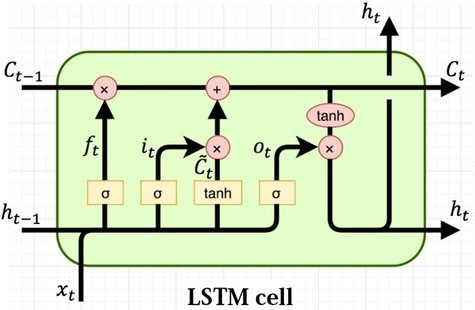
\includegraphics[width=0.5\linewidth]{LSTM.jpeg}
\end{center}

\textbf{Example}
Depending on the weights, the input $\mathbf{x}_{(t)}$ could have only a small effect on $y_{(t)}$ but a large effect on the long term memory $C_{(t)}$ and thus also on later outputs $y_{(t+n)} (n>1)$.

\newpar{}
\ptitle{Remarks}
\begin{itemize}
    \item [+] LSTM models solve the problem of vanishing gradients
    \item [+] easier to preserve information of many time steps (cell learns when to remember $h$ and when to forget it)
\end{itemize}
